% This is "sig-alternate.tex" V2.0 May 2012
% This file should be compiled with V2.5 of "sig-alternate.cls" May 2012
%
% This example file demonstrates the use of the 'sig-alternate.cls'
% V2.5 LaTeX2e document class file. It is for those submitting
% articles to ACM Conference Proceedings WHO DO NOT WISH TO
% STRICTLY ADHERE TO THE SIGS (PUBS-BOARD-ENDORSED) STYLE.
% The 'sig-alternate.cls' file will produce a similar-looking,
% albeit, 'tighter' paper resulting in, invariably, fewer pages.
%
% ----------------------------------------------------------------------------------------------------------------
% This .tex file (and associated .cls V2.5) produces:
%       1) The Permission Statement
%       2) The Conference (location) Info information
%       3) The Copyright Line with ACM data
%       4) NO page numbers
%
% as against the acm_proc_article-sp.cls file which
% DOES NOT produce 1) thru' 3) above.
%
% Using 'sig-alternate.cls' you have control, however, from within
% the source .tex file, over both the CopyrightYear
% (defaulted to 200X) and the ACM Copyright Data
% (defaulted to X-XXXXX-XX-X/XX/XX).
% e.g.
% \CopyrightYear{2007} will cause 2007 to appear in the copyright line.
% \crdata{0-12345-67-8/90/12} will cause 0-12345-67-8/90/12 to appear in the copyright line.
%
% ---------------------------------------------------------------------------------------------------------------
% This .tex source is an example which *does* use
% the .bib file (from which the .bbl file % is produced).
% REMEMBER HOWEVER: After having produced the .bbl file,
% and prior to final submission, you *NEED* to 'insert'
% your .bbl file into your source .tex file so as to provide
% ONE 'self-contained' source file.
%
% ================= IF YOU HAVE QUESTIONS =======================
% Questions regarding the SIGS styles, SIGS policies and
% procedures, Conferences etc. should be sent to
% Adrienne Griscti (griscti@acm.org)
%
% Technical questions _only_ to
% Gerald Murray (murray@hq.acm.org)
% ===============================================================
%
% For tracking purposes - this is V2.0 - May 2012

\documentclass{sig-alternate}
\usepackage{fixltx2e}
\usepackage{xcolor}
\def\SPSB#1#2{\rlap{\textsuperscript{\textcolor{red}{#1}}}\SB{#2}}
\def\SP#1{\textsuperscript{\textcolor{black}{#1}}}
\def\SB#1{\textsubscript{\textcolor{black}{#1}}}
\newenvironment{myquote}
               {\list{}{\rightmargin   \leftmargin
                        \parsep        0in }%
                \item\relax}
               {\endlist}
\newcommand{\userquote}[2]{\begin{samepage}\begin{myquote} 
     \em{\small{#2\begin{flushright}---#1\end{flushright}}}
   \end{myquote}\end{samepage}}
%Quote code
%\newif\ifquoteopen
%\catcode`\"=\active % lets you define `"` as a macro
%\DeclareRobustCommand*{"}{%
%   \ifquoteopen
%     \quoteopenfalse ''%
%   \else
%     \quoteopentrue ``%
%   \fi
%}

%End of quote code

\begin{document}
\setlength{\parindent}{0pt}
\CopyrightYear{2016}
\setcopyright{acmcopyright}
\conferenceinfo{ACM DEV '16,}{Nov 18-21, 2016, Nairobi, Kenya}
%\isbn{978-1-4503-4306-0/16/06}\acmPrice{\$15.00}
%\doi{http://dx.doi.org/10.1145/2909609.2909664}
%
% --- Author Metadata here ---
%\conferenceinfo{ICTD'16}{June 3-6 2016, Ann Arbor, Michigan, USA}
%\CopyrightYear{2007} % Allows default copyright year (20XX) to be over-ridden - IF NEED BE.
%\crdata{0-12345-67-8/90/01}  % Allows default copyright data (0-89791-88-6/97/05) to be over-ridden - IF NEED BE.
% --- End of Author Metadata ---

%\title{Alternate {\ttlit ACM} SIG Proceedings Paper in LaTeX
%\title{Leveraging on Families' Social Interactions on Utilization of Personal Health Informatics through Intermediaries}
\title{A Family Wellness App: Engage Children to Manage Wellness of Adults}
%
% You need the command \numberofauthors to handle the 'placement
% and alignment' of the authors beneath the title.
%
% For aesthetic reasons, we recommend 'three authors at a time'
% i.e. three 'name/affiliation blocks' be placed beneath the title.
%
% NOTE: You are NOT restricted in how many 'rows' of
% "name/affiliations" may appear. We just ask that you restrict
% the number of 'columns' to three.
%
% Because of the available 'opening page real-estate'
% we ask you to refrain from putting more than six authors
% (two rows with three columns) beneath the article title.
% More than six makes the first-page appear very cluttered indeed.
%
% Use the \alignauthor commands to handle the names
% and affiliations for an 'aesthetic maximum' of six authors.
% Add names, affiliations, addresses for
% the seventh etc. author(s) as the argument for the
% \additionalauthors command.
% These 'additional authors' will be output/set for you
% without further effort on your part as the last section in
% the body of your article BEFORE References or any Appendices.

\numberofauthors{3} %  in this sample file, there are a *total*
% of EIGHT authors. SIX appear on the 'first-page' (for formatting
% reasons) and the remaining two appear in the \additionalauthors section.
%
\author{
% You can go ahead and credit any number of authors here,
% e.g. one 'row of three' or two rows (consisting of one row of three
% and a second row of one, two or three).
%
% The command \alignauthor (no curly braces needed) should
% precede each author name, affiliation/snail-mail address and
% e-mail address. Additionally, tag each line of
% affiliation/address with \affaddr, and tag the
% e-mail address with \email.
%
% 1st. author
\alignauthor
        Ntwa Katule \\
        \affaddr{University of Cape Town}\\
        \affaddr{Department of Computer Science}\\
        \affaddr{Cape Town, South Africa}\\
        \email{katulentwa@gmail.com}
% 2nd. author
\alignauthor
Melissa Densmore\\
        \affaddr{University of Cape Town}\\
        \affaddr{Department of Computer Science}\\
        \affaddr{Cape Town, South Africa}\\
        %\affaddr{Institute for Clarity in Documentation}\\
        %\affaddr{P.O. Box 1212}\\
        %\affaddr{Dublin, Ohio 43017-6221}\\
        \email{mdensmore@cs.uct.ac.za}
% 3rd. author
\alignauthor Ulrike Rivett\\
        \affaddr{University of Cape Town}\\
        \affaddr{Department of Information Systems}\\
        \affaddr{Cape Town, South Africa}\\
        \email{ulrike.rivett@uct.ac.za}
       %\affaddr{The Th{\o}rv{\"a}ld Group}\\
        %\affaddr{1 Th{\o}rv{\"a}ld Circle}\\
        %\affaddr{Hekla, Iceland}\\
        %\email{larst@affiliation.org}
%\and  % use '\and' if you need 'another row' of author names
% 4th. author
%\alignauthor Lawrence P. Leipuner\\
%       \affaddr{Brookhaven Laboratories}\\
%       \affaddr{Brookhaven National Lab}\\
%       \affaddr{P.O. Box 5000}\\
%       \email{lleipuner@researchlabs.org}
% 5th. author
%\alignauthor Sean Fogarty\\
%       \affaddr{NASA Ames Research Center}\\
%       \affaddr{Moffett Field}\\
%       \affaddr{California 94035}\\
%       \email{fogartys@amesres.org}
% 6th. author
%\alignauthor Charles Palmer\\
%       \affaddr{Palmer Research Laboratories}\\
%       \affaddr{8600 Datapoint Drive}\\
%       \affaddr{San Antonio, Texas 78229}\\
%       \email{cpalmer@prl.com}
}
% There's nothing stopping you putting the seventh, eighth, etc.
% author on the opening page (as the 'third row') but we ask,
% for aesthetic reasons that you place these 'additional authors'
% in the \additional authors block, viz.
%\additionalauthors{Additional authors: John Smith (The Th{\o}rv{\"a}ld Group,
%email: {\texttt{jsmith@affiliation.org}}) and Julius P.~Kumquat
%(The Kumquat Consortium, email: {\texttt{jpkumquat@consortium.net}}).}
\date{30 July 1999}
% Just remember to make sure that the TOTAL number of authors
% is the number that will appear on the first page PLUS the
% number that will appear in the \additionalauthors section.

\maketitle 

\begin{abstract} 
The pandemic of lifestyle-related chronic diseases has led to an advent of personal health informatics, with the goal of persuading individuals to adopt healthful lifestyles. Such systems implement various motivational affordances to promote ongoing use. Design of such systems focuses in engaging only the beneficiary of information derived from those systems. In this study we explored how one can use gamification to motivate ongoing usage of such systems in the context of intermediated technology use. We studied the effect of gamification in motivating young family members in assisting adults who might be less conversant or intimidated with such a technology. We compared two designs of a mobile wellness application of which one prototype was gamified and the other one was not gamified. Our findings suggest that virtual rewards can enhance usage of such systems through intermediary users. We highlight some of the design implications in order to foster perceived enjoyment in using such a system.    
\end{abstract}
%
% The code below should be generated by the tool at
% http://dl.acm.org/ccs.cfm
% Please copy and paste the code instead of the example below. 
%

\begin{CCSXML}
<ccs2012>
<concept>
<concept_id>10002944.10011122.10002947</concept_id>
<concept_desc>General and reference~General conference proceedings</concept_desc>
<concept_significance>500</concept_significance>
</concept>
<concept>
<concept_id>10003120.10003121.10011748</concept_id>
<concept_desc>Human-centered computing~Empirical studies in HCI</concept_desc>
<concept_significance>300</concept_significance>
</concept>
<concept>
<concept_id>10003456.10010927</concept_id>
<concept_desc>Social and professional topics~User characteristics</concept_desc>
<concept_significance>100</concept_significance>
</concept>
</ccs2012>
\end{CCSXML}

\ccsdesc[500]{General and reference~General conference proceedings}
\ccsdesc[300]{Human-centered computing~Empirical studies in HCI}
\ccsdesc[100]{Social and professional topics~User characteristics}

%
% End generated code
%

%
%  Use this command to print the description
%
\printccsdesc


%A category including the fourth, optional field follows...
\keywords{HCI4D, intermediated interactions, persuasive technologies, gamification, personal informatics, motivational affordances, health}

\section{Introduction} 
Lifestyle-related diseases are now attracting many players seeking to design low cost and tailored information and communications technology (ICT)- based systems for supporting lifestyle change and disease management\cite{arsand:mobile} with most recent development focusing in persuasive technlogies. A systematic review of 95 studies on persuasive technologies found out that persuasive systems have the capability to persuade because their design include implementation of persuasion stimuli \cite{hamari2014persuasive}.\newline
Persuasive systems include personal informatics which can be used for persuasion of health behaviours. Personal informatics systems are interactive applications that support users to become self-aware of patterns in the behaviours, by providing means to collect personal history, as well as tools for its review or analysis \cite{li2011:personal,li2012:personal}. Persuasion stimuli in a personal informatics rely on their ability to support reflective learning/self-reflection \cite{li2011:understanding}. Reflective learning entails reviewing of collected personal data to learn about oneself and the user always alternates between two phases known as discovery of a behaviour pattern and maintenance of a better behaviour\cite{li2011:understanding}. These phases are usually supported through feedback mechanisms such as bar charts or other affective mechanisms such as gardens that represent steps walked (i.e Ubifit\cite{klasnja2009:using}) or Fish growing or shrinking depending to an increase or decrease in the number of steps walked (i.e Fish'nSteps \cite{lin2006:fish}). The aforementioned techniques can further be supplemented with social comparison\cite{Oinas-kukkonen:psd} or competitions with others \cite{comber2013:designing} in some systems. General approaches on how to design such systems have been proposed with ideas coming from both HCI\cite{li2010:stage} and persuasive technologies fields \cite{fogg2009:behavior,Oinas-kukkonen:psd,Oinas-Kukkonen:foundation}.  \newline
However utilization of such systems may be constrained to specific demographics such as young or experienced users of technology. For instance , one study evaluated two of the popular fitness apps, Nike+ and RunKeeper, and concluded that the two apps are not ready to accommodate older adults needs \cite{silva2014:smartphones}. In addition to that, in developing countries there are scenarios of intermediated technology use for users who are inexperience or intimidated by technology and many of the existing apps are designed to accommodate only direct users of technology \cite{sambasivan2010}. Therefore, in personal health informatics, features that foster ongoing use are targeted towards beneficiaries of the information processed by the app. But in the context of intermediated technology there is an intermediary user who is there to facilitate access of information to beneficiary users hence that facilitator needs to also be motivated to support ongoing use of a personal health informatics.\newline
In our work, we replicate the idea of intermediated technology use into personal health informatics as we believe that it can support users who are less conversant in technology. Instead of just involving an adult beneficiary user in interacting with a personal health informatics, we bring young family members to become part of the interaction process and apply gamification to foster ongoing use. One study found out that perceived interest to use gamification decreases with age and this implies that such a gamified system might be more effective if utilized through younger populations\cite{v2014motivational}.\newline
In this study we report on the outcome of using gamification and how different it is in comparison to involving intermediaries without gamification. We also propose approaches that can enhance the impact of gamification in the context of personal health informatics used through intermediary users.
\section{Related Work} 
Zhang et al.\cite{zhang2008:motivational} suggested a list of motivational affordances that could be implemented in a system in order to foster its usage such as: (1) the system should afford self-identity and autonomy;(2) the system should support provision of challenges/competitions; (3)the system should allow users to relate to each other; etc. The aforementioned motivational affordances must be fulfilled in order to support the three basic psychological needs that are suggested by a self-determination theory (SDT) and these are: (1) the need for autonomy; (2)the need for challenges/competitions that are developmentally appropriate;  (3) the need to belong to a group \cite{deci1985:intrinsic}. Individuals engage in activities to satisfy the aforementioned psychological needs \cite{deterding2011:situated}. The support for the three needs is important for a person to feel intrinsically motivated to perform a certain task.\newline     
Personal health informatics have been designed with specific motivational affordances to engage users with their personal data. For instance a personal informatics with just a self-monitoring feature can provide afford the need for challenges as users set goals and challenge themselves to attain those goals. Literature in public health also recognizes goal setting as an important part towards health behaviour change~\cite{strecher1995goal}. Other motivation affordances that support competitions and relatedness with others can be implemented to support the process of self-monitoring. But these motivational affordances are usually implemented to motivate a beneficiary user alone hence it is challenging to motivate ongoing use in the context where a beneficiary user has to to rely on an intermediary user to interact with his/her personal data.
The phenomenon of young people providing support to adults on technological related problems is quite prevalent in both HCI and ICTD literature. Studies have explored factors influencing help-seeking and giving behaviours and have pointed out factors such group orientations towards tasks unfamiliarity with technology, social rapport,reciprocal benefits, the sense of being accountable and many others to play a significant role in mediating help-seeking and help giving behaviors in various contexts.\cite{sambasivan2010,poole:chh,kiesler:twi,parikh2006}. However the aforementioned literature in intermediated technology use is limited to general use of technology and it has not focused on specialized technology such as a personal health informatics which has received a lot of attention within HCI community. In our work, we designed a system that allows an intermediary user and a beneficiary user to work together to sustain ongoing use of the system.\newline
In order to engage the two sets of users with the system and foster its ongoing use, we implemented game design elements. The two users worked as a pair to form a team of where any virtual rewards are specifically awarded to a team and not an individual user. Gamification is an idyllic avenue that is used in engaging users with personal informatics or persuasive technology targeting health behaviour change because of its ability to trigger intrinsic experiences \cite{hamari2014persuasive}. Gamification borrows game design mechanics such as points, leader-boards, badges, etc in non-game contexts. It brings together the motivation pull from video games. The motivation pull behind video games is due to its support for the three construct of self-determination theory \cite{ryan2006:motivationalpull}. Gamification has been found to have a potential to address motivational mechanisms and thereby fosters motivation \cite{sailer2013:psychological}. The aforementioned psychological needs can be supported with game design elements.\newline
The use of gamification has been studied in tasks such as image annotation\cite{mekler2013:points,mekler2013:disassembling},crowd reporting\cite{crowley2012:gamification}, data collection \cite{cechanowicz2013:effects} etc. and not in intermediated information tasks. The intermediated information task is different from the other tasks as there may be two users collaborating to engage with a user interface with the goal of one user assisting another user with his/her information needs. For the case of personal informatics, motivational affordances need to motivate the two users to work together in engaging with the system. Perceived interest/enjoyment in gamification tends to diminish with increasing in age \cite{v2014motivational} and this suggests that young people are the perfect choice for intermediaries. We limited selection of intermediary users to family members because in our previous study we observed that familial relationships were the key to the success of such an intervention.\newline 
Our main research question attempts to understand the effectiveness of gamification in facilitating usage through intermediary users.
\section{Methods}
\subsection{Participants' Demography}
Participants for this study were recruited from Langa and Athlone, two of the many townships in Cape Town, South Africa. Majority of the households in these two townships fall under the bracket of low income earners in South Africa. The recruitment was facilitated one research assistant and her field work who reside in Langa and Athlone respectively.\newline
A total of fourteen adult participants were recruited with mean age of 44.21 years(S.D of 9.99 years). The youngest adult was 26 years of age while the oldest was 60 years of age. Thirteen of these adult participants were females. Each adult participant elected one of their children/grand children to work with. The two members of a pair were required to work together in using the ``Family Wellness App'' to self-monitor the wellness of an adult member of a pair (a beneficiary). The average age of children participants was 15.42 (S.D=2.06) years. The youngest intermediary participants was 12 years of age while the oldest was 20 years of age. The number of females and males intermediary participants were equal. Prior to be part of the study all adult participant signed consent forms and also all children participant sign an assent form which was also signed by their respective adult participants.\newline  
\subsection{Experiment Design}
\begin{figure}
\centering
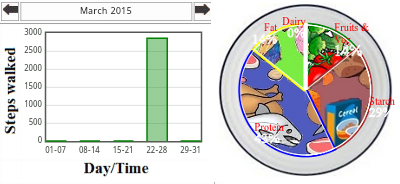
\epsfig{file=logbookapp.png, height=1.5in, width=3in}
\caption{Screen-shots showing logbook features: step bar chart and meal pie chart}
\label{figure:logbookapp}
\end{figure}
\begin{figure}
\centering
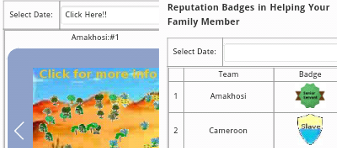
\epsfig{file=gameapp.png, height=1.5in, width=3in}
\caption{Screen-shots showing badges and a fitness garden}
\label{figure:gameapp}
\end{figure}
We were comparing two versions of the "Family Wellness App". The first version of the application was simply a logbook or journal (Figure \ref{figure:logbookapp}) that allows each pair of participants to view steps graphs and recording and viewing summaries of nutrition components of food consumed by a beneficiary within a pair. The second version also contained all the aforementioned features of logbook with an added gamification component (Figure \ref{figure:gameapp}). A gamification component consisted of a leader board (points' score board), badges,avatars, message board, botanical gardens, and fish tanks (aquarium). The rules for rewards were were as follows:
\begin{itemize}
\item{\textbf{Points}}:Points are earned by an average number of steps/per day walked by a beneficiary participant are added to usage points. Each day of app usage is equivalent to 1000 usage points.
\item{\textbf{Badge}}: There were a total of 10 ranked badges. The highest badge was ranked number 1 while the lowest was ranked number 10. To attain a badge that is one step higher than the current badge, there were certain fixed requirements and these are; a pair has to use the app for a minimum number of days required for attaining that badge, and a beneficiary member of a pair needs to have walked a minimum average of number of steps specified for that particular badge. 
\item{\textbf{Botanical garden}}: A botanical garden had trees on one side and flowers on the other side. Number of trees is determined by the corresponding rank of badge while the size is determined by the number of meals recorded by a pair divided the number of meals of a pair with the highest number. Suppose a pair ``P'' has a badge that is ranked number \emph{`n'}.  The number of trees in a garden for a pair P will be as shown on Equation \ref{equation:numtrees}. Suppose the tree is ``z'' when it is big enough, then then the size of each tree for a pair P is determined by Equation \ref{equation:sizetrees} of where \emph{`a'} is the total number of meals recorded by pair P ,\emph{`b'} is the highest number of meals recorded by a particular pair lets ''Q'',\emph{`c'} is the ratio of fruits and vegetables in all meals that have been recorded by pair P before, and z is either height or width of a tree when it has grown up to the maximum size( width=50 pixels; height=50 pixels).   For instance pair has a badge that is ranked number 7 will have (10-7) multiply by 10= 30 trees. Lets assume this pair recorded a total of a=7 meals or which its overall nutritions components constitutes of c=0.3 from fruits and vegetables. Also lets assume that a pair that had recorded the highest number of meals had a total of b=12 meals. Then the size of each tree will be; height=((7/12)*height of a tree when it is big enough)+0.3;width=((7/12)*width of a tree when it is big enough)+0.3.  Flowers are determined by the overall usage of the system in number of days. In each day of app usage, a pair receives 10 flowers. The size of each flower is also determined by the Equation \ref{equation:sizetrees}
\begin{equation}
\label{equation:numtrees}
y=((10-n)*10) 
\end{equation}
\begin{equation}
\label{equation:sizetrees}
y=((a/b)*z)+c 
\end{equation}
\item{\textbf{Fish Tanks}}: The rules for garden were the same rules used to determine how many fish will be present in the tank and their sizes. In our previous informative evaluation reported in one study we observed that these rules can actually motivate  intermediaries to use the app and also to persuade their beneficiary participant to live healthy. Ideas that use visualizations similar to the fish tank and botanical garden have been previously studied in HCI \cite{klasnja2009:using,lin2006:fish}
\end{itemize} 
There is no systematic procedure of how we arrived to the aforementioned rules. These rules were just arbitrary.  We just invented them based on insights from a preliminary evaluation of the gamified prototype.\newline
Both versions of the systems implemented reminders. In the logbook version, SMS were sent to remind intermediary participants to assist their respective beneficiary participants in self-monitoring of their steps and diet. In addition, those logbook reminders consisted of the current average number of steps walked per day by a beneficiary participant since the first day of using the app. In the gamified version, SMS were sent to remind pairs what they need to do in order to achieve rewards, and also what they have done so far (current status), and what remains to be done in order to attain a much higher status. For instance children can be reminded that recording more fruits and vegetable from their parents will give them a better botanical garden.\newline    
In order to compare the two versions of the system, the experimental design was within group which uses the same group of participants to test both system: (1)logbook only; and (2) the one that includes both logbook and gamified components. In order to minimize the impact of the learning effect on one experimental condition,each pair of participant was randomly assigned to one of the two experimental sequences. The first sequence consisted of individual pairs of participants that started with the logbook version and finished with the gamified version. This sequence is referred to as ``LG'' group. The second sequence  consisted of individual pairs of participants that started with the gamified version and finished with the logbook version. This sequence is referred to as ``GL'' group. A total of seven pairs of participants were assigned to the LG group while the remaining seven pairs were assigned to the GL group. 
\subsection{Data collection} 
Prior to data collection each intermediary participant from the 14 pairs was given an android phone that they could use with their adult participants. Each pair of participants was allocated 1.3 GB of data to use through the duration of experiments. In addition each beneficiary participant was given a total of ZAR 240 (approx. US \$20) as a compensation for transport and their time for the duration of the study.\newline
We carried out this evaluation for a period of six weeks starting from Mid October 2015 running up to the last week of November 2015. The first four weeks were spent on logbook version for the ``LG'' group and  gamified version for the ``GL'' group. Thereafter, pairs in LG group were switched to gamified version while pairs in ``GL'' group were switched to logbook. Both versions of the app were used for two weeks after the aforementioned switching.\newline
We collected data through triangulation of usage logs for the two versions of the prototype,intrinsic motivation inventory(IMI) questionnaires, and interviews. We developed the IMI questionnaires with guidance of materials found on a ``Self-Determination Theory''\footnote{http://www.selfdeterminationtheory.org/intrinsic-motivation-inventory/} website which is maintained by researchers working on the theory including Richard Ryan and Edward Deci\cite{deci1985intrinsic} whom were early pioneers in developing the theory. These questionnaires were pretested in one of our early pilot studies.\newline
There were two sets of questionnaires, one for adult (beneficiaries) participants , and another one for children (intermediaries)  participants. Both questionnaires were administered at three points: (1) baseline (before experiments); (2) midline (the fourth week, before switching of experimental conditions; (3) endline (after concluding usage experiment at the end of the sixth week).\newline
The baseline questionnaire for the intermediary participants assesses the perceived enjoyment of intermediaries in helping other people with cellphone related tasks. The midline questionnaire for the intermediary participants assesses the ability of the two prototype to support the three basic psychological needs postulated by the self-determination theory: (1) autonomy, (2) competence, and (3) relatedness. Therefore we selected three sub-scales from the IMI questionnaire and these were (1)perceived autonomy, (2) perceived competence, and (3) perceived relatedness. The endline questionnaire for intermediaries was the same as the midline one.\newline
The baseline questionnaur
\section{Discussion}
\section{Conclusions}


%\end{document}  % This is where a 'short' article might terminate

%ACKNOWLEDGMENTS are optional 

\section{Acknowledgments} 

.

%
% The following two commands are all you need in the
% initial runs of your .tex file to
% produce the bibliography for the citations in your paper.
%small{
\bibliographystyle{abbrv}
\bibliography{sigproc} %} % sigproc.bib is the name of the Bibliography in this case
% You must have a proper ".bib" file
%  and remember to run:
% latex bibtex latex latex
% to resolve all references
%
% ACM needs 'a single self-contained file'!
%
%APPENDICES are optional
%\balancecolumns


\end{document}
